	\tikzstyle{decision} = [diamond, draw, fill=blue!20, 
	text width=4.5em, text badly centered, node distance=3cm, inner sep=0pt]
	\tikzstyle{block} = [rectangle, draw, fill=cyan!50, 
	text width=8em, text centered, rounded corners, minimum height=4em]
	\tikzstyle{line} = [draw, -latex']
	\tikzstyle{cloud} = [draw, ellipse,fill=red!20, node distance=3cm,
	minimum height=2em]

		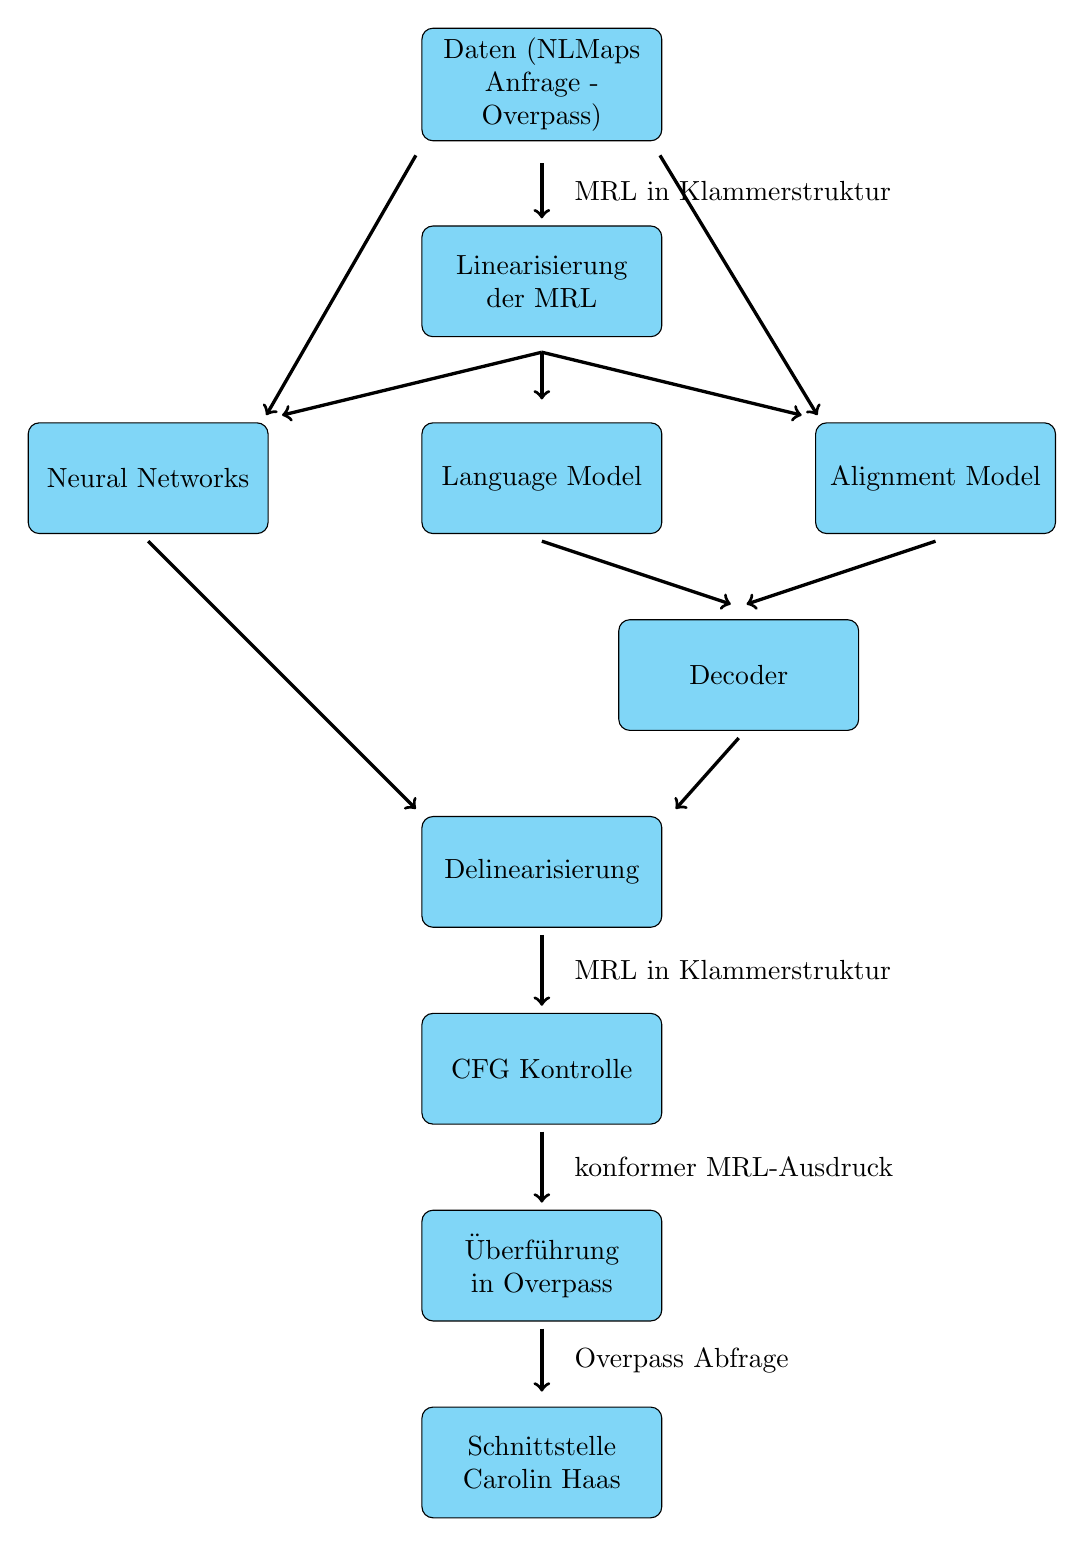
\begin{tikzpicture}[node distance = 2cm, auto]
		% Place nodes
		
		\node [block] at (6 ,9) (daten){Daten (NLMaps Anfrage - Overpass)};
		\node [block] at (6 ,6.5) (linear){Linearisierung der MRL};
		\node [block] at (1 ,4) (neural){Neural Networks};
		\node [block] at (6 ,4) (language){Language Model};
		\node [block] at (11 ,4) (align){Alignment Model};
		\node [block] at (8.5, 1.5) (decoder){Decoder};
		\node [block] at (6, -1) (delinear){Delinearisierung};
		\node [block] at (6 ,-3.5) (cfg){CFG Kontrolle};
		\node [block] at (6 ,-6) (overpass){\"Uberf\"uhrung in Overpass};
		\node [block] at (6 ,-8.5) (schnitt){Schnittstelle Carolin Haas};	
		% Draw edges
		\draw[->, very thick] (6,8) --  node[label= right:MRL in Klammerstruktur] {} (6,7.3);
		\draw[->, very thick] (4.4,8.1) --  node[] {} (2.5,4.8);
		\draw[->, very thick] (7.5,8.1) --  node[] {} (9.5,4.8);
		\draw[->, very thick] (6,5.6) --  node[] {} (6,5);
		\draw[->, very thick] (6,5.6) --  node[] {} (2.7,4.8);
		\draw[->, very thick] (6,5.6) --  node[] {} (9.3,4.8);
		\draw[->, very thick] (6,3.2) --  node {} (8.4,2.4);
		\draw[->, very thick] (11,3.2) --  node {} (8.6,2.4);
		\draw[->, very thick] (1,3.2) --  node {} (4.4,-0.2);
		\draw[->, very thick] (8.5,0.7) --  node {} (7.7,-0.2);	
		\draw[->, very thick] (6,-1.8) --  node[label=right:MRL in Klammerstruktur] {} (6,-2.7);	
		\draw[->, very thick] (6,-4.3) --  node[label= right: konformer MRL-Ausdruck] {} (6,-5.2);
		\draw[->, very thick] (6,-6.8) --  node[label=right: Overpass Abfrage] {} (6,-7.6);
		
		\end{tikzpicture}